% !TEX root = MAIN.tex

\chapter{\DAMA - Validation Execution Environment Definition and Results}

\begin{figure}[h]
  \centering
  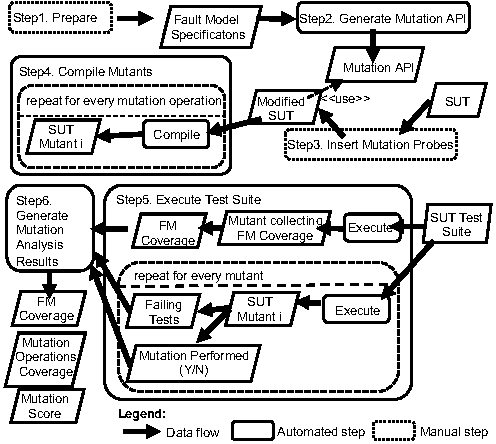
\includegraphics[width=0.6\textwidth]{images/dataDrivenBufferProcess.pdf}
      \caption{DAMAt methodology.}
      \label{fig:damat}
\end{figure}

Figure~\ref{fig:damat} introduces \DAMA methodology.
Validation was performed by applying the \DAMA methodology to the case studies listed in the \emph{SPAP} document (chapter 5):
\begin{itemize}
  \item LXS System Test Suite for ESAIL.
  \item GSL System Test Suite for LibParam.
\end{itemize}

Particularly, we verified that \DAMA complied with the requirements expressed in the \emph{Software System Specification} (\emph{SSS}), section 4.1.1.
To this purpose, two validation approaches were devised:
\begin{itemize}
  \item Unit Testing
  \item Application to Case Studies
\end{itemize}

These approaches are composed of validation tasks as laid out in Table~\ref{table:damat:results} (Application to Case Studies) and Table~\ref{table:damat:unit_results}.

The aforementioned tables also include the results as of Monday 20/09/2021.

The validation tasks are described in details in the \emph{Software Validation Specification} (\emph{SVS}) document, Chapter 5.

A detailed description of \DAMA unit testing is available in the \emph{Software Unit Test Plan} (\emph{SUTP}) (Chapters 11, 12, 13, and 14) and a detailed report in the \emph{Software Unit Test Report} (Chapters 6 and 7).

\begin{table}[h]
\caption{\DAMA Validation Report, Unit Testing.}
\label{table:damat:unit_results}
\scriptsize
\centering
\begin{tabular}{|l|l|l|l|}
\hline
\textbf{Validation Approach}&\textbf{Task}&\textbf{Result}\\
\hline
Unit Testing&Performing \emph{DAMAt-TD-DDMutation-1}&PASSED\\
Unit Testing&Performing \emph{DAMAt-TD-DDMutation-2}&PASSED\\
% Application to Case Studies&Instrumenting the source code - \DAMA&PASSED&PASSED\\
% Application to Case Studies&Configuring and running \emph{\DAMA\_compile.sh} Application to Case Studies&PASSED&PASSED\\
% Application to Case Studies&Configuring and running \emph{\DAMA\_run\_test.sh}&PASSED&PASSED\\
% Application to Case Studies&Configuring and running \emph{\DAMA\_obtain\_coverage.sh}&PASSED&PASSED\\
% Application to Case Studies&Configuring and running \emph{\DAMA\_mutants\_launcher.sh}&PASSED&PASSED\\
\hline
\end{tabular}

\end{table}


\begin{table}[h]
\caption{\DAMA Validation Report, Application to Case Studies}
\label{table:damat:results}
\scriptsize
\centering
\begin{tabular}{|l|l|l|l|}
\hline
\textbf{Validation Approach}&\textbf{Task}&\textbf{ESAIL}&\textbf{libparam}\\
\hline
% Unit Testing&Performing \emph{DAMAt-TD-DDMutation-1}&PASSED&PASSED\\
% Unit Testing&Performing \emph{DAMAt-TD-DDMutation-2}&PASSED&PASSED\\
Application to Case Studies&Instrumenting the source code - \DAMA&PASSED&PASSED\\
Application to Case Studies&Configuring and running \emph{\DAMA\_compile.sh} Application to Case Studies&PASSED&PASSED\\
Application to Case Studies&Configuring and running \emph{\DAMA\_run\_test.sh}&PASSED&PASSED\\
Application to Case Studies&Configuring and running \emph{\DAMA\_obtain\_coverage.sh}&PASSED&PASSED\\
Application to Case Studies&Configuring and running \emph{\DAMA\_mutants\_launcher.sh}&PASSED&PASSED\\
\hline
\end{tabular}

\end{table}





% Particularly, we verified that \DAMA was able to:
% \begin{enumerate}
% 	\item Parse a fault model prepared by the user.
% 	\item Generate a mutation API with the functions that modify the data according to the provided fault model.
%   \item Modify the buffer through calls to the mutation API.
% 	\item Generate and compile mutants.
% 	\item Execute the test suite against all the mutants and gather the results of the test cases.
% 	\item Generate the results of the mutation analysis.
% \end{enumerate}

% \begin{table}[h]
% \caption{MASS Validation Report.}
% \label{table:damat:results}
% \scriptsize
% \centering
% \begin{tabular}{|@{\hspace{1pt}}p{33mm}|
% @{\hspace{1pt}}>{\raggedleft\arraybackslash}p{12mm}@{\hspace{1pt}}|
% >{\raggedleft\arraybackslash}p{12mm}@{\hspace{1pt}}|
% >{\raggedleft\arraybackslash}p{12mm}@{\hspace{1pt}}|
% >{\raggedleft\arraybackslash}p{12mm}@{\hspace{1pt}}|
% }
% \hline
% \textbf{Methodology Step}&\textbf{ESAIL}&\textbf{libgscsp}&\textbf{libparam}\\
% \hline
% Parse the fault model&PASSED&PASSED&PASSED\\
% Generate the mutation &PASSED&PASSED&PASSED\\
% Modify the buffer&PASSED&PASSED&PASSED\\
% Generate and compile the mutants&PASSED&PASSED&PASSED\\
% Execute the test suite&PASSED&PASSED&PASSED\\
% Generate the results&PASSED&PASSED&PASSED\\
% \hline
% \end{tabular}
%
% \end{table}
%
% The idea was to verify that every step of the methodology produced the correct input/outputs. For this reason, we provide Table~\ref{table:damat:results}, that shows the success/failure of every \DAMA step on the different case studies.
%
% A detailed exposition of the validation results is presented in the \emph{D4} document (Chapter 2).

\clearpage
